\section{Рабочий проект}
\subsection{Классы, используемые при разработке сайта}

Можно выделить следующий список классов и их методов, использованных при разработке web-приложения (таблица \ref{class:table}).

\renewcommand{\arraystretch}{0.8} % уменьшение расстояний до сетки таблицы
\begin{xltabular}{\textwidth}{|X|p{2.5cm}|>{\setlength{\baselineskip}{0.7\baselineskip}}p{4.85cm}|>{\setlength{\baselineskip}{0.7\baselineskip}}p{4.85cm}|}
\caption{Описание классов, используемых в приложении\label{class:table}}\\
\hline \centrow \setlength{\baselineskip}{0.7\baselineskip} Название класса & \centrow \setlength{\baselineskip}{0.7\baselineskip} Модуль, к которому относится класс & \centrow Описание класса & \centrow Методы \\
\hline \centrow 1 & \centrow 2 & \centrow 3 & \centrow 4\\ \hline
\endfirsthead
\caption*{Продолжение таблицы \ref{class:table}}\\
\hline \centrow 1 & \centrow 2 & \centrow 3 & \centrow 4\\ \hline
\finishhead
AdminLogin & Главный модуль & AdminLogin – является наследником класса View из модуля templatesview.baseview. Класс AdminLogin предоставляет метод get, который используется для обработки HTTP GET-запросов на определенный URL. & при вызове метода get для объекта класса AdminLogin, он вернет HTML-код, сгенерированный из указанного шаблона templates/adminlogin.

html. Этот код, используется для отображения страницы входа в админ-панель при обработке GET-запроса по соответствующему URL.\\
\hline AdminView & Главный модуль & AdminView – является наследником класса View из модуля templatesview.baseview. Класс AdminView предоставляет метод get, который используется для обработки HTTP GET-запросов на определенный URL. & при вызове метода get для объекта класса AdminView, он вернет HTML-код, сгенерированный из указанного шаблона templates/admin.html. Этот код используется для отображения страницы админ-панели при обработке GET-запроса по соответствующему URL.\\

\hline View(ABC) & Главный модуль & View(ABC) – определяет абстрактный базовый класс View, который наследуется от ABC (Abstract Base Class). & класс View служит базовым классом для других классов представлений и предоставляет атрибут template, который потомки могут использовать для указания пути к своим HTML-шаблонам. Однако, для полноценного абстрактного класса, скорее всего, потребуется дополнительное определение абстрактных методов или свойств.\\

\hline HomeView & Главный модуль & HomeView – является наследником класса View из модуля templatesview.homeview. Класс HomeView предоставляет метод get, который используется для обработки HTTP GET-запросов на определенный URL. & при вызове метода get для объекта класса HomeView, он вернет HTML-код, сгенерированный из указанного шаблона templates/home.html. Этот код используется для отображения страницы админ-панели при обработке GET-запроса по соответствующему URL.\\

\hline ImageView & Главный модуль & HomeView – является наследником класса View из модуля templatesview.imageview. Класс ImageView предоставляет метод get, который используется для обработки HTTP GET-запросов на определенный URL. & при вызове метода get для объекта класса ImageView, он вернет HTML-код, сгенерированный из указанного шаблона templates/images.html. Этот код используется для отображения страницы админ-панели при обработке GET-запроса по соответствующему URL.\\

\end{xltabular}
\renewcommand{\arraystretch}{1.0} % восстановление сетки

\subsection{Системное тестирование разработанного web-сайта}

На рисунке \ref{main:image} представлена главная страница сайта портфолио фотографа.
\newpage % при необходимости можно переносить рисунок на новую страницу
\begin{figure}[H] % H - рисунок обязательно здесь, или переносится, оставляя пустоту
\center{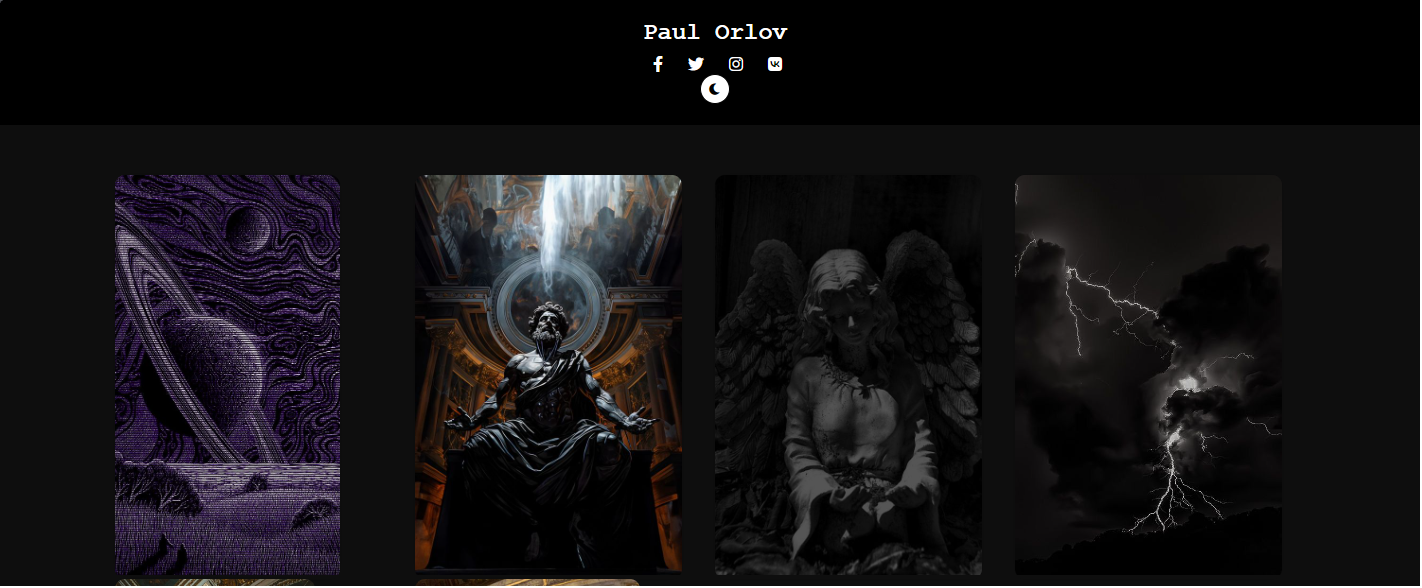
\includegraphics[width=1\linewidth]{main1}}
\caption{Главная страница сайта портфолио фотографа.}
\label{main:image}
\end{figure}

На рисунке \ref{menu:image} представлена страница фотографии.

\begin{figure}[ht]
\center{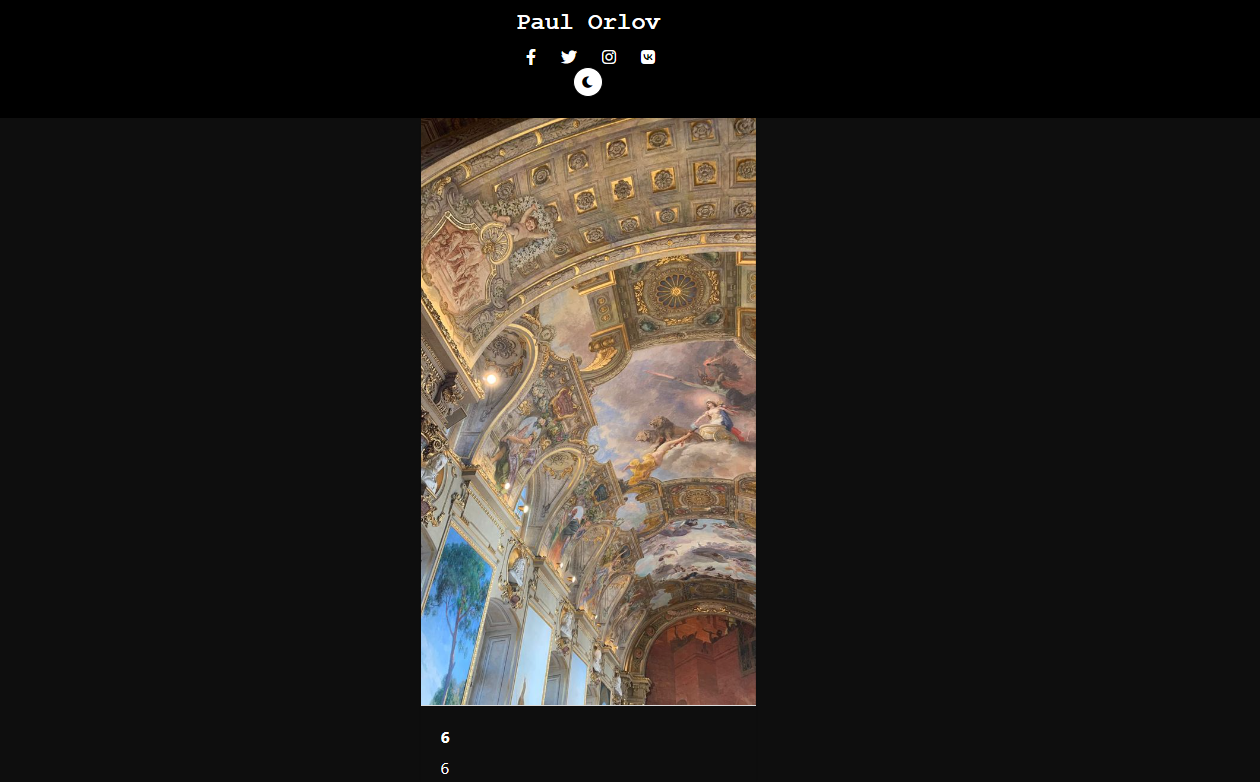
\includegraphics[width=1\linewidth]{menu}}
\caption{Страница фотографии}
\label{menu:image}
\end{figure}

\newpage
На рисунке \ref{enter:image} представлена страница авторизации в административную панель.

\begin{figure}[ht]
\center{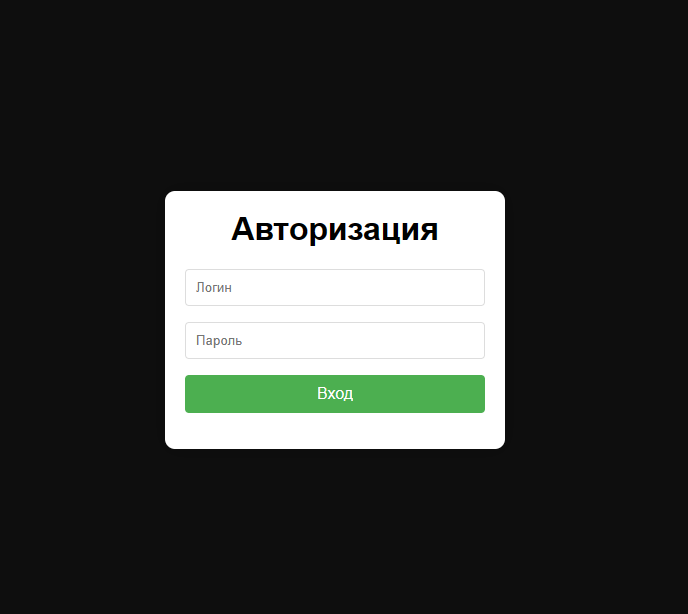
\includegraphics[width=1\linewidth]{enter}}
\caption{Страница авторизации}
\label{enter:image}
\end{figure}

\newpage
На рисунке 4.4 представлена страница административной панели.

\begin{figure}[ht]
	\center{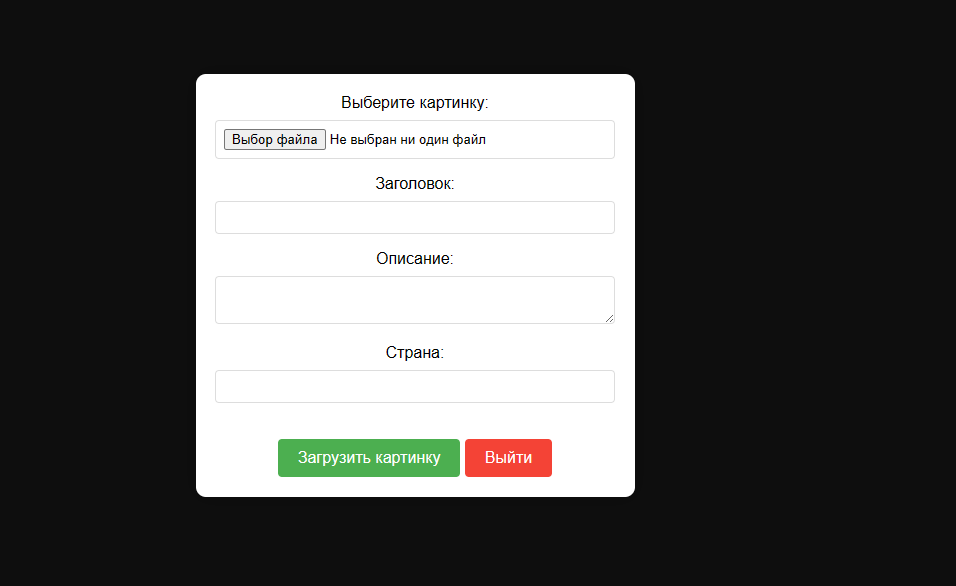
\includegraphics[width=1\linewidth]{add}}
	\caption{Страница добавления изображения}
	\label{add:image}
\end{figure}
